\documentclass[crop,class=article]{standalone}
%----------------------------Preamble-------------------------------%
\usepackage{amsfonts}                   % Blackboard Bold R.
\usepackage{tikz}                       % Drawing/graphing tools.
\usetikzlibrary{arrows.meta}            % Latex and Stealth arrows.
%--------------------------Main Document----------------------------%
\begin{document}
    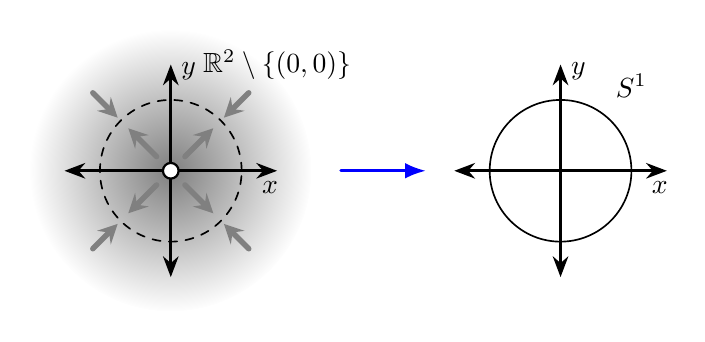
\begin{tikzpicture}[%
        scale=0.9,
        line width=1pt,
        line cap=round,
        >={Stealth[black]},
        every edge/.style={%
            draw=black,
            very thick
        },
        grayarrow/.style={%
            >=stealth,
            fill=gray,
            draw=gray,
            line width=0.7mm,
            ->
        }
    ]
        \filldraw[%
            even odd rule,
            inner color=gray,
            outer color=white,
            draw=white
        ]
            (0,0) circle (2);

        % Draw axes.
        \draw[<->] (-1.5,0) -- (1.5,0);
        \draw[<->] (0,-1.5) -- (0,1.5);
        \draw[<->] (4,0) -- (7,0);
        \draw[<->] (5.5,-1.5) -- (5.5,1.5);

        % Draw gray arrows indicating homotopy equivalence.
        \begin{scope}[every edge/.style=grayarrow]
            \draw(1.1,1.1) edge (0.75,0.75);
            \draw(-1.1,-1.1) edge (-0.75,-0.75);
            \draw(1.1,-1.1) edge (0.75,-0.75);
            \draw(-1.1,1.1) edge (-0.75,0.75);
            \draw(0.2,0.2) edge (0.6,0.6);
            \draw(-0.2,-0.2) edge (-0.6,-0.6);
            \draw(0.2,-0.2) edge (0.6,-0.6);
            \draw(-0.2,0.2) edge (-0.6,0.6);
        \end{scope}

        \draw[dashed,draw=black,semithick] (0,0) circle (1);
        \node[%
            fill=white,
            circle,
            thick,
            draw,
            inner sep=2pt,
            outer sep=3pt
        ]
            at (0,0) (O) {};
        \node at (1.4,0) [below] {$x$};
        \node at (0,1.4) [right] {$y$};
        \node at (1.5,1.5) {$\mathbb{R}^{2}\setminus\{(0,0)\}$};
        \draw[>=Latex,draw=blue,->] (2.4,0) -- (3.6,0);
        \draw[draw=black,semithick] (5.5,0) circle (1);
        \node at (6.9,0) [below] {$x$};
        \node at (5.5,1.4) [right] {$y$};
        \node at (6.5,1.2) {$S^{1}$};
    \end{tikzpicture}
\end{document}